\documentclass[11pt,a4paper]{article}
%\usepackage{beamerarticle}

%\usefonttheme[onlymath]{serif}
\usepackage[ngerman]{babel}
\usepackage[utf8]{inputenc}
\usepackage[T1]{fontenc}
\usepackage{tikz}
\usetikzlibrary{positioning, arrows}
\usepackage{listings}
\usepackage{fancybox}
\usepackage{color}
\usepackage{hyperref}
\usepackage{fancyhdr}

\pagestyle{fancy}
\lhead{\today}
\rhead{Author: Fabian Tronicke}
\chead{Gruppe: swp15.gkp}
%\cfoot{center of the footer!}
\renewcommand{\headrulewidth}{0.8pt}
%\renewcommand{\footrulewidth}{0.4pt}

\begin{document}
\center \large Universität Leipzig - Softwaretechnik Praktikum 2014/2015\\
\center \Huge Entwurfsbeschreibung zum Vorprojekt \\
\par\bigskip

\small zum Projekt: Ein kartenbasiertes “Multiplayer”-Spiel

\par\bigskip

\tableofcontents

\clearpage

\flushleft
\section{Allgemeines}
Im Rahmen des SWT-Praktikums wird ein kartenbasiertes Multiplayerspiel entwickelt, das es ermöglicht, ein an das alte Pacman angelehnte Computerspiel auf einem realen Kartenausschnitt zu spielen.
Im Vorprojekt wird eine kleine Web Applikation erstellt, welche die Architektur minimal implementiert und eine einfache Interaktion mit der Karte ermöglicht.
Genauer gesagt ist es möglich einen Spielort auszuwählen und dort mit einer Spielfigur über den Kartenausschnitt zu laufen, sowie mit einer weiteren Spielfigur zu interagieren.

\section{Produktübersicht}
Der Nutzer kann online über die Spiele-Website auf das Programm zugreifen.
Dabei stehen dem Nutzer ein Suchfeld zum finden der gewünschten Spielumgebung zur Verfügung, die Möglichkeit die Spielfigur zurück zusetzen und die Lautstärke über einen Regler anzupassen.
Hat man den Ort ausgewählt, kommt eine weitere Spielfigur (der Geist) ins Spiel, die sich zufallsgeneriert über die Karte bewegt.
Man kann die Spielfigur, den Pucman, nun steuern und wenn man es schafft mit Pucman den Geist einzufangen, wird ein Geräusch ausgelöst.
Während des Spielens werden die Möglichkeiten zur Veränderung der Kartenansicht deaktiviert um sicherzustellen, dass der Spieler sich nicht unabsichtlich vom Spielgeschehen entfernen kann.
Das ganze Spielgeschehen ist durch einen Soundtrack unterlegt, der eine  funktionale und inhaltliche Verbindung zwischen Bild und Musik  generiert.
Desweiteren befinden sich bereits Platzhalter für den späteren Highscore, die verbleibende Anzahl an Leben und die Möglichkeit direkt auf die Website des Spiels zugreifen zu können.

\section{Grundsätzliche Struktur- und Entwurfsprinzipien}
Die von uns umgesetzte Web-Anwedung basiert auf einer Client-Server Archiketkur.  Beim Server liegen die Daten, die vom Client abgefragt werden und an diesem übertragen werden. Die Googlemaps API stellt alle wichtigen Funktionen zur Verfügung, GameBlock Javascript 
\begin{figure}[htb]
  \centering
  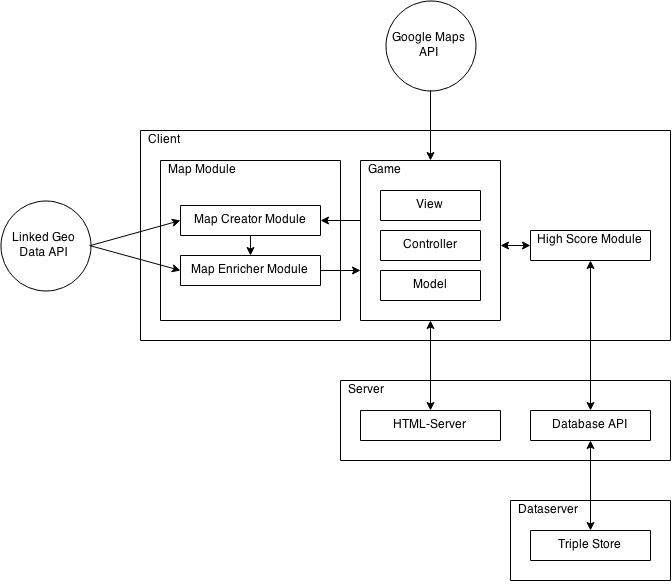
\includegraphics[scale=0.5]{arch.png}
%\caption{der rote Punkt bezeichnet unser gesuchtes Teilwort}
  \label{PNFs}
\end{figure} 



\section{Struktur- und Entwurfsprinzipien der einzelnen Pakete}
\section{Datenmodell}
 
\section{Testkonzept}
Alle nötigen Funktionen werden von der Google Maps Api bereitgestellt.
Aufgrund des einfachen Programmaufbaus verzichten wir daher für das Vorprojekt auf ein besonderes Testkonzept und führen stattdessen manuelle Tests in Hinsicht auf die Funktionalität durch.
\section{Glossar}
Das Glossar wurde überarbeitet und als externes Dokument angefügt.
\end{document}